% !TEX root = ../lifeonbrane3.tex
%

We have described a holographic framework where quantum extremal surfaces and the island rule \reef{wonderA} can be examined in higher dimensions, \ie for gravity theories in $d\ge2$. In particular, the background is simple enough that the construction given in section \ref{sec:branegravity} is straightforward and purely analytic, in contrast to the numerical approach of \cite{Almheiri:2019psy}. In section \ref{face}, we were also able to describe the system from three different perspectives, analogous to the three descriptions of the two-dimensional system examined in \cite{Almheiri:2019hni}. In particular, we have the boundary perspective, where the system is described as a $d$-dimensional CFT coupled to a ($d-1$)-dimensional conformal defect;
the bulk gravity perspective, where ($d+1$)-dimensional gravity with a negative cosmological constant is coupled to a codimension-one brane; and the brane perspective, where the boundary CFT is coupled to an AdS$_d$ region which supports Einstein gravity and two copies of the same CFT, which are weakly coupled to each other. As we emphasized, this last perspective is an effective theory, as is made clear by the cut-off arising in this Randall-Sundrum braneworld scenario. As discussed and examined in some detail in section \ref{HEE}, this effective gravity theory lends itself to the appearance of quantum extremal islands in the brane perspective, although these have a conventional interpretation from the bulk gravity perspective, in terms of RT surfaces which cross the brane for certain of choices of the entangling geometry on the boundary.\\

\hd{Unconventional features:} Of course, the analysis presented in our paper is somewhat unusual in that we are finding quantum extremal islands but there are no black holes, no horizons and no Hawking radiation involved. Rather we simply considered the entanglement entropy of various entangling regions in the vacuum state of the boundary system. However, to favour the formation of these quantum extremal islands, and at the same time have the brane in the `Einstein gravity regime,' \ie $L/\leff\ll1$, we had to introduce somewhat unconventional couplings. That is, we considered a negative Newton's constant on the brane $\lamb<0$ and nonzero Gauss-Bonnet coupling $\lgb$ for a four-dimensional bulk. Both of these choices were enhancing the connected RT surfaces over the disconnected RT surfaces in calculating the holographic EE. Of course, an interesting question is the interpretation of these `exotic' bulk couplings in terms of data describing the boundary CFT (and the conformal defect). While we do not have a precise interpretation, some qualitative results can be stated.

As observed in section \ref{face}, using standard holographic techniques, one finds that the gravitational coupling in the DGP brane action \reef{newbran} affects the spectrum of defect operators in the boundary theory \cite{domino}. Now let us reiterate that there is no apriori reason not to consider $\lamb<0$. For example, integrating out quantum fields on the brane could produce either a positive or negative shift of Newton's constant. In particular, the shift can be negative for gauge fields or nonminimally coupled scalar fields, as was discussed in the context of EE in \cite{Larsen:1995ax,Kabat:1995eq} -- see also discussion is appendix \ref{bubble}. However, this scenario is not the one we are describing here. In particular, additional brane fields such as these would make significant contributions to the EE which are not accounted for in our calculations. Hence, implicitly, we simply assume that the gravitational coupling $1/\Gbr$ (either positive or negative) is induced by some unknown UV physics.

Introducing the Gauss-Bonnet term \reef{top2} does not modify the gravitational dynamics in the four-dimensional bulk, considered in section \ref{sec:examples}, and hence the correlators of the stress tensor are not modified in the dual three-dimensional boundary theory.\footnote{Of course, such modifications arise for holographic constructions in higher dimensions \cite{Buchel:2009sk}.} However, the topological coupling $\lgb$ affects the entanglement structure of the boundary CFT states. To see this, consider calculating the entanglement entropy holographically for two nearby regions in the boundary. The phase transition between connected and disconnected phase of the RT surfaces is sensitive to a Gauss-Bonnet term. For positive $\lgb$, the transition from disconnected to connected phase takes place earlier (and vice versa for negative $\lgb$). This means that with $\lgb>0$, the mutual information between these two regions remains of order $c_\mt{T}$ for larger separations, \eg \cite{Headrick:2010zt}. Note, however, that choosing positive $\lgb$ favours higher genus surfaces. A concern with this choice might be if higher genus extremal surfaces exist, they may produce unusual results. Finally, we note that the topological coupling appears directly in the expressions for the holographic EE, \eg see eq.~\reef{Sdisc}. Therefore to have an appreciable effect, we must choose this coupling to be of the order of the central charge of the boundary theory, \ie $\lgb\sim L^2/\Gbk\sim \cT$.

Let us add that in section \ref{sec:examples}, we focused on the example of $d=3$ with a four-dimensional bulk. In this case, the natural topological term to add to the bulk gravity is the Gauss-Bonnet term \reef{top2}. Of course, the scenario extends straightforwardly to any $d=2n-1$ for which there is a corresponding topological term which can be added to the bulk gravity action, \ie the Euler character for $2n$-dimensional manifolds, \eg see \cite{Hung:2011xb}. Similarly, for even boundary dimensions ($d=2n$), the analogous topological terms could be added to the brane action, where they would not modify the dynamics of gravity on the brane but they would modify the gravitational entropy associated with the boundary of the quantum extremal islands. 

In light of these unconventional features, a natural question therefore is whether we find quantum extremal islands in our analysis with both $\lamb =0= \lgb$. The answer is affirmative, however, one must reduce to the tension of the brane to reduce its backreaction and the extent of the additional geometry in the vicinity of the  brane's location. As a result, the connected RT surfaces will have a smaller (bulk) area contribution as they cross the brane. However, in this case, the curvature of the AdS geometry on the brane is also smaller, and hence the effective description of the brane theory in terms of Einstein gravity breaks down. That is, with $\leff\sim L$, the contributions of the higher curvature corrections in the induced action \reef{act3} are no longer suppressed relative to the Einstein term and these new interactions play an important role in the dynamics of gravity in the brane perspective. Furthermore, the cutoff of the corresponding CFT on the brane will be much lower. Alternatively, one could think about computing the EE in settings beyond the vacuum state that we studied here. In fact, in \cite{QEI}, we will explicitly show without additional Gauss-Bonnet or DGP couplings that quantum extremal islands appear for (nonextremal) eternal black holes in equilibrium with an external heat bath, \ie in a higher dimensional analog of the analysis in \cite{Almheiri:2019yqk}.

Let us conclude here by comparing our approach with the recent work \cite{Geng:2020qvw}, which appeared while the present paper was prepared for submission. The latter examines essentially the same model (with no DGP term) but concentrates on a very different regime. The authors of \cite{Geng:2020qvw} focused on the formation of islands for the case of a tensionless brane, where the brane gravity becomes very nonstandard, as explained above. Further, in the limit where the graviton becomes massless, \ie $\ell_\mt{eff}\to \infty$, they  observe that no islands form \cite{Geng:2020qvw}. On the other hand, the present work focuses the regime of large brane tension, where the theory on the brane can be well approximated by Einstein gravity (\ie the graviton mass and higher curvature interactions are negligible). We moreover show that by allowing either a topological term or a negative $\Gbr$, islands can appear even in the absence of horizons.\\ 

\hd{Resolving Puzzles:} Our construction clarifies certain conceptual puzzles that arose in early discussions of quantum extremal islands in a holographic framework, \eg for the two-dimensional gravity models introduced in \cite{Almheiri:2019hni} and studied in \cite{Almheiri:2019yqk, Chen:2019uhq}. For example in these models the Planck brane, which supports the JT gravity theory, appears at the boundary of the three-dimensional bulk spacetime. Hence one might have wondered if the brane degrees of freedom (including the JT gravity) are a part of the boundary theory or part of the bulk theory. In our construction, the Planck brane is in the middle of the spacetime geometry and so this question does not arise -- these degrees of freedom belong to the bulk. An important corrolary of this observation is that when a quantum extremal island appears on the brane, \eg see the lower panel in figure \ref{fig:RTPhases}, we are able to recover information about the island with data from the boundary CFT in the corresponding boundary subregion, by applying standard entanglement wedge reconstruction \cite{EW1,EW2,EW3,Jafferis:2015del,Dong:2016eik,Faulkner:2017vdd,Cotler:2017erl}. Of course, the latter would not apply if the brane degrees of freedom were a part of the boundary theory.

Further, our construction circumvents the question of whether RT surfaces are allowed to end on the Planck brane. Rather in our paper, the extremal surfaces just pass through the bulk and only end on the asymptotic boundary as usual. It is simply that in certain situations, the RT surfaces will pass through the brane, which of course, corresponds to the formation of a quantum extremal island.

Another `novel' feature of the two-dimensional JT gravity model of \cite{Almheiri:2019hni} was that the holographic entanglement entropy included an extra boundary term, \ie the gravitational entropy of the JT model, where the RT surface terminated on the Planck brane. That is, the holographic entanglement entropy was given by extremizing the sum of the bulk area of the RT surface and this additional boundary term. An analogous gravitational entropy term on the brane arises in our construction with a DGP brane -- see eq.~\reef{eq:sad}. In fact, our derivation in appendix \ref{generalE} suggests that if the brane supports intrinsic gravitational interactions then the corresponding Wald-Dong entropy on the brane is part of the holographic entanglement entropy formula, as shown in eq.~\reef{fish9}. Hence this general result agrees with the boundary term introduced in the two-dimensional JT gravity models, mentioned above. A shortcoming of the derivation in appendix \ref{generalE} is that the geometric configuration involved a high degree of symmetry, which precluded  finding the expected extrinsic curvature terms \cite{Dong:2013qoa}. Therefore it would be interesting to extend our construction there to more general configurations  along the lines of \cite{Lewkowycz:2013nqa,Dong:2016hjy}.

We want to emphasize the above discussion is distinct from finding in section \ref{sec:enzyme} that the leading contribution to the holographic EE where the RT surface crosses the brane matches the Wald-Dong entropy of the induced gravitational action on the brane\reef{act3}.\footnote{Recall that this analysis was general enough to see the extrinsic curvature contributions coming from the higher curvature interactions in eq.~\reef{act3}.} For example, the leading contribution is $\area(\sigma_\xR)/{4G_\mt{eff}}$, where $\sigma_\xR$ is the cross-section of the RT surface on the brane. As shown in eq.~\reef{eq:bazinga2}, the DGP term is one important contribution to this result, but the bulk area of the RT surface in the vicinty of the brane is also necessary. Of course, we still find the leading contributions reproduce the gravitational entropy of the induced gravity theory on the brane even without the DGP term, \ie with $1/\Gbr=0$. This must be closely related to the fact that the bulk Einstein equations combined with the Israel junction conditions are equivalent to the gravity equations of motion on the brane in the Randall-Sundrum scenario \cite{deHaro:2000wj}.

In passing we note here that $d=2$ is distinguished in the above discussion. In this case, the leading contribution corresponds to the Wald-Dong entropy for the the Polyakov-Liouville action \eqref{PolyAct2} and takes the form given in eq.~\reef{arc}. However, since it only depends on the curvature scalar which is constant across the AdS$_2$ geometry of the brane, this contribution takes the same value no matter where the RT surface  crosses the brane. This contrasts with the higher dimensional result $\area(\sigma_\xR)/{4G_\mt{eff}}$, which rapidly grows as the position of $\sigma_\xR$ moves to larger radii on the brane. That is, there is an enormous penalty against forming large quantum extremal islands for $d\ge3$. In contrast, no such penalty arises for $d=2$ facilitating the formation of islands, as discussed in detail in
\cite{Rozali:2019day}. Of course, if one adds JT gravity \reef{JTee} to the two-dimensional brane action, as in eq.~\reef{braneact2}, then the gravitational entropy on the brane includes $\(\Phi_0+
\Phi(x)\)/4\Gbr$, which will favour smaller quantum extremal islands because the dilaton profile grows with the radius on the brane \cite{Maldacena:2016upp}.

Of course, we can modify our higher dimensional construction to make it more analogous to the two-dimensional model introduced in \cite{Almheiri:2019hni} by taking a $\mathbb Z_2$ orbifold quotient across the brane. With this orbifold, the brane appears as the edge of the bulk geometry but clearly the association with the bulk degrees of freedom has not changed. The brane now only supports a a single copy of the boundary CFT and there are factors of 1/2 appearing in various expressions, \eg we make the following replacement in eq.~\reef{Newton2}: ${1}/{G_\mt{eff}}=L/((d-2)\Gbk)$. Similarly, the RT surfaces will now end on the orbifolded brane while satisfying the boundary condition,
\beq\label{ortho8}
 0  =  \tg_j{}^\nu\(g_{\mu\nu}\,\partial_{n}X^\mu
  + \frac{G_\bulk}{G_\brane}\,\inducedK_i \,\partial_\nu x^i\)\,,
\eeq
%\rcm{Vincent: please confirm}\vc{I'm not sure about the factor of 2: if there are really two identical bulks, then \eqref{ortho8} is just a special case of \eqref{ortho7} and the factor of 2 is correct; but, if there is only one bulk (as suggested by stripping off a factor of $2$ in \eqref{Newton2} to get ${1}/{G_\mt{eff}}=L/((d-2)\Gbk)$ mentioned above), then the $\partial_{n_L} X^\mu$ term in \eqref{ortho7} is just not present, so there should not be a factor of 2 in \eqref{ortho8}.}
which replaces eq.~\reef{ortho7}. Further, the conformal defect becomes a conformal boundary in the orbifolded theory, \ie the spatial geometry on which the CFT lives is now a ($d-1$)-dimensional hemisphere with the conformal boundary being the $S^{d-2}$ at the edge of the hemisphere. 

Other questions that may have arisen from the early discussions of quantum extremal islands which focussed on JT gravity might include the importance of having a low spacetime dimension, \ie $d=2$, or of the JT model itself. The early work of \cite{Penington:2019npb} considered black hole evaporation with Einstein gravity in higher dimensions, and the holographic model of \cite{Almheiri:2019hni} was extended to a holographic framework with $d=4$ in \cite{Almheiri:2019psy} using numerical calculations. Hence our paper reinforces these results by describing quantum extremal islands in a new setting, in particular, in higher dimensions and with Einstein gravity. Our construction is also simple enough that further investigations of the role of quantum extremal islands in higher dimensions are straightforward, \eg see \cite{QEI}. Let us add that JT gravity can be seen as the gravitational dual of the so-called SYK model \cite{Maldacena:2016hyu,Sachdev:1992fk,Sachdev:2010um,Ktalks}. This duality involves an ensemble average over the couplings in the boundary quantum mechanics and so one may expect that this averaging plays a role in the appearance of quantum extremal islands. However, it seems that this is not the case as our construction relies on the standard holographic rules of the AdS/CFT correspondence where there is no such averaging of the couplings in the boundary theory.

One other perplexing issue with the island rule \reef{rule1} is the appearance of the entanglement of the CFT degrees of freedom in the region $\CFTR$ on both sides of the equation \cite{Almheiri:2019hni}. As explained in \cite{Almheiri:2019yqk}, we should distinguish the ``full quantum description'' of, \eg the Hawking radiation in the presence of black holes on the left-hand side from the ``semiclassical description'' which includes the outgoing radiation and purifying partners on the quantum extremal island on the right-hand side. Our holographic construction makes clear that the description of quantum states with islands in the brane picture is on a different footing than that solely in terms of the boundary theory. In particular, referring to the three perspectives discussed in section \ref{face}, it is clear that the boundary perspective (with the boundary CFT coupled to a conformal defect) gives a complete description of quantum state.  By the standard rules of the AdS/CFT correspondence, the bulk perspective (where Einstein gravity with a negative cosmological constant is coupled to a codimension-one brane) gives an equivalent description.\footnote{In this paper, we modeled the CFT defect with a simple brane in the bulk. This bottom-up approach is neither sufficient, nor completely correct. For example, in the case of $\mathcal N=4$ SYM theory on $S^4$, the presence of an interface breaks at least half of the supersymmetry generators and the $R$ symmetry. In a complete description, this will result in a deformation of the bulk $S^5$. For top-down models, see \cite{Karch:2001cw,DeWolfe:2001pq, DHoker:2007hhe, DHoker:2008rje, Chiodaroli:2009yw, Chiodaroli:2011nr, Chiodaroli:2012vc}. }
However, the brane perspective has a different character. In particular, the description in terms of a CFT coupled to the dynamical AdS$_d$ region is only an effective one. Indeed, as emphasized in section \ref{face}, the Randall-Sundrum gravity is only valid down to  the short distance cutoff $\tilde\delta\sim L$, \ie see eqs.~\reef{ctoffplus} and \reef{ctoffminus}. Beyond this cutoff, gravity is no longer localized to the brane and the additional `Kaluza-Klein' modes of the graviton are strongly coupled to the brane and their contribution cannot be ignored. 

Further, this brane perspective also provides an effective description of the coupling to the defect CFT. That is, it only accounts for the couplings localized at the defect, which dominate at low energies, but ignores the subtle nonlocal couplings, which could be seen as coming through the bulk AdS geometry in the dual description. Of course, the quantum extremal islands in the effective description of the brane perspective are a clear example of this. These islands are a remnant of replica wormholes in the limit $n\to1$ \cite{Penington:2019kki,Hartman:2020swn}. However, in the replica trick construction of the corresponding Renyi entropies in the bath CFT, one can ask why the gravity on the different branes in the replica copies should connect with one another. However, these effective gravity theories are UV completed by a single theory of gravity in the bulk and so it is natural to consider geometries connecting the branes, \ie replica wormholes if the effective theory. Hence the connection of the brane and boundary through the bulk provides a simple explanation of these wormholes.  Given the simplicity of our construction, it may provide a useful framework in which to understand further subtleties in distinguishing the various expressions in the island rule.

As a final note here, we observe that the finite cutoff for the CFT on the brane has noticeable effects even for $d=2$, \eg see eq.~\reef{almost}. In contrast, the early discussions of \eg \cite{Almheiri:2019hni,Almheiri:2019psf, Almheiri:2019yqk, Chen:2019uhq, Penington:2019kki, Almheiri:2019qdq} assumed that one could use standard formulae for conformal transformations in the $d=2$ CFT in the gravitational region (\ie on the brane). It would be interesting to understand if the cutoff modifies any of this analysis in a significant way \cite{QEI}.\\

\hd{Brane geometry, Part I:} As described in section \ref{sec:branegravity}, we choose the brane tension to produce a negative cosmological constant in the gravity theory on the brane, in accord with eqs.~\reef{act3} and \reef{Newton2}. As a result, the $d$-dimensional geometry on the brane is AdS space. However, it is straightforward to consider the case where the brane tension takes its critical value, such that $1/\ell_\mt{eff}^2=0$, as is usually done in the Randall-Sundrum scenario \cite{Randall:1999ee,Randall:1999vf}. In this case, the analogous brane geometry is simply flat space, and the brane is easily embedded in the bulk AdS$_{d+1}$ geometry on a slice of constant radius (or constant $z$) in standard Poincar\'e coordinates. An interesting feature of this embedding is that the brane reaches the asymptotic AdS$_{d+1}$ boundary along the null boundaries of the flat space geometry (as well as a timelike and spacelike infinity) \eg see \cite{Karch:2001cw}. 
%\dn{I've added Karch-Randall as a ref, since they draw nice pictures (see figure 5 in ''locally localized gravity''. However, I don't think there is an explicit reference which discusses these constructions in detail. It seems to always have been common knowledge.} 
Hence we can naturally investigate quantum extremal surfaces and the island formula in flat space using the usual expressions for holographic entanglement entropy in this construction as long as we consider regions on null infinity. Notably this matches the approach pursued in \cite{Hartman:2020swn}, but contrasts with studies of \eg \cite{Gautason:2020tmk} which considered spacelike regions. It would, of course, be interesting to use this framework to study quantum extremal islands in the context of asymptotically flat braneworld black holes, \eg as described in \cite{Emparan:1999wa,Emparan:1999fd}. We should note however that there are undoubtedly subtleties with the proposed construction, \eg as the brane completely cuts out the asymptotic AdS$_{d+1}$ boundary (except for a single point) on constant time slices. 

Of course, one can also consider the case where the brane tension is chosen such that $1/\ell_\mt{eff}^2<0$. That is, the brane gravity theory would have a positive cosmological constant and the corresponding brane geometry becomes de Sitter space. In this case, one constructs a foliation of the bulk AdS$_{d+1}$ geometry in terms of $d$-dimensional de Sitter slices and the brane can be embedded along the slice with the appropriate curvature, \eg see \cite{Karch:2001cw}. In this case, the brane reaches the asymptotic AdS$_{d+1}$ boundary on the future and past timelike infinities of the de Sitter geometry. 
%\dn{Don't know of any reference, but again seems like common knowledge.} 
Hence, this construction provides a framework to use holographic entanglement entropy for investigating the island formula in de Sitter space as long as we consider regions on the timelike future of the latter geometry. Let us add that this would be similar to upcoming work of \cite{dSone,dStwo}, which studies related questions in the context of JT gravity with a positive cosmological constant 
\cite{Maldacena:2019cbz}. The de Sitter evolution of the Hartle-Hawking vacuum prepares a two-dimensional CFT state on circle and the entanglement entropy of various regions in the latter state are investigated, revealing new islands in the de Sitter geometry \cite{dSone,dStwo}.\\ 
%\dn{I'm not sure what the last sentence refers to.}\\

\hd{Brane geometry, Part II:}



The geometry of the setup presented in this paper might look unconventional. As seen from the brane perspective, we have the bath CFT on the asymptotic boundary with geometry $S^{d-1} \times \mathbb R$, and two copies of the same CFT on the brane with an AdS$_d$ geometry. These two geometries are joined by introducing a cutoff surface (with topology $S^{d-2} \times \mathbb R$) near the asymptotic boundary of the AdS$_d$ geometry and gluing it to the equator of the  $S^{d-1} \times \mathbb R$ geometry. In particular, the resulting geometry is not a manifold in the vicinity of the gluing region -- see the left panel of figure \ref{fig:no_mfld}. Of course, we can obtain a manifold by taking the $\mathbb Z_2$ quotient which identifies the two halves of the bath CFT, such that the theory is again defined on a manifold with topology $S^{d-1} \times \mathbb R$. However, we will ignore this simplification here. Rather, we want to comment on the theory before taking the $\mathbb Z_2$ quotient. 

\begin{figure}[t]
\centering
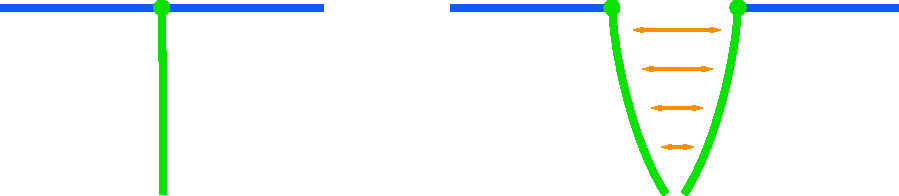
\includegraphics[scale = 0.7]{no_mfld}
\caption{Left: In the brane perspective, the bath CFT on the asymptotic boundary (blue) is connected to two copies of the effective CFT on the brane (green) but the resulting geometry is not a manifold. Right: For excitations below the effective CFT cutoff the system behaves as if it consists of two systems on a manifold which are weakly coupled in the gravitational region (green).}
\label{fig:no_mfld}
\end{figure}

First, we note that constructions where multiple CFTs are joined at a common defect are not rare. For example they appear in the study of boundary and interface CFTs (\eg see \cite{Chiodaroli:2012vc}), and sometimes seem to be required to remove anomalies \cite{Ooguri:2020sua}.

Second, we would like to argue that in the regime where the defect theory can be described by two copies of the boundary CFT coupled to Einstein gravity, we can approximately think of the full theory as two copies of the orbifolded theory (each living on a manifold), which are weakly coupled in the gravitational region -- see the right panel of figure \ref{fig:no_mfld}. This is particularly easy to see from the bulk perspective. For brevity we restrict ourselves to the discussion of graviton modes, but a similar story applies to all bulk fields. 

Let us begin by recalling that for $\veps \ll 1$, the spectrum of graviton fluctuations in the bulk is almost unchanged with respect to the modes in (two copies of) empty AdS space. Hence much of the corresponding physics should be very similar that of two copies of the the AdS$_{d+1}$, or to two copies of the dual CFT$_d$ on the boundaries of two independent AdS$_{d+1}$ geometries. Of course, one exception to the preceding is that upon gluing the two AdS$_{d+1}$ geometries together, a new set of very light graviton states localized in the vicinity of the brane \cite{Randall:1999vf,Randall:1999ee,Karch:2000ct,Karch:2001jb}, as discussed in section \ref{face}. For simplicity, we refer to the latter as the brane graviton modes, while we refer to the former as the standard normalizable modes.\footnote{These bulk modes are $\mathbb Z_2$ graded under reflection across the Planck brane, and the even modes survive the $\mathbb Z_2$ orbifold discussed above include the brane graviton states as well as half of the standard normalizable modes. However, this organization of the modes is not useful for the following discussion.}

On a fixed time slice, as shown in the right panel of figure \ref{fig:brane2}, the standard normalizable modes will describe stress energy excitations in the dual CFT on both the left and right halves of the asymptotic boundary. If we assume an approximate extrapolate dictionary \cite{Harlow:2011ke} for the brane theory as well, these normalizable modes will also describe analogous excitations for the effective CFT on the brane. However, there will be two sets of such excitations: those described by bulk excitations\footnote{We stress here that the localized excitations considered here do not correspond to individual energy eigenmodes, which were implicit in the previous paragraph. Rather they will consist of linear combinations of such eigenmodes evaluated on the fixed time slice being examined here. Of course, having superpositions of energy eigenmodes is what produces the complicated time evolution described below.} with support primarily in the right copy of the AdS$_{d+1}$ geometry, and those described by the analogous excitations primarily in the left AdS$_{d+1}$ geometry. Hence, the stress tensor on the brane can be decomposed into two pieces which correspond to subsectors of the brane theory, each of which is determined by bulk excitations which essentially live on one side of the brane. If these subsectors were truly superselection sectors (\eg as one might imagine arises in the limit $\veps\to0$), our brane theory would contain two independent copies of the boundary CFT  and each of these copies would only interact with the bath CFT on the corresponding half of the asymptotic boundary. That is, each of these systems would live on an independent manifold with topology $S^{d-1} \times \mathbb R$. 

However, this is not strictly correct and the two copies of the CFT on the brane are weakly coupled with $\veps\ll1$ but finite. In particular, localized stress energy excitations of the form considered above will not remain localized with time evolution. Rather they will eventually spread across the entire asymptotic boundary if time evolves for a sufficiently long time. For example, an excitation localized on the right asymptotic boundary will evolve to eventually produce excitations of the stress tensors on the left asymptotic boundary and on the brane as well. From the boundary perspective, excitations moving onto the brane correspond to excitations that are absorbed by the conformal defect (and remain there for a long time).

The spreading of the localized excitations can be seen to arise through two physical effects: First, the bulk excitations can tunnel between the two AdS$_{d+1}$ regions shown in figure \ref{fig:brane2}. Recall that (the radial part of) the linearized bulk equation of motion can be reduced to a Schroedinger equation with a double-well potential, where the height of the barrier is determined by the brane tension \cite{Karch:2000ct}. With $\veps\ll1$ but finite, the barrier height while large remains finite and there will be a finite probability for a bulk excitation on one side of the Planck brane to tunnel to the other. A second independent coupling comes because the stress tensors of the two copies of the CFT couple to the same gravity theory on the brane. From the bulk perspective, the nonlinear Einstein equation produces interactions between the brane graviton modes with excitations on either side of the brane. Hence bulk excitation excitations on one side can leak to the other side by scattering process involving the brane gravitons. However, we note that both effects become smaller as the brane tension approaches its critical value, \ie as $\veps$ approaches zero. Thus, to a good approximation, the brane theory can be treated at two copies of the boundary CFT which only interact weakly. \\


\hd{Entanglement wedge cross-sections:} Recent work \cite{Takayanagi:2017knl,Nguyen:2017yqw} has drawn attention to
the entanglement wedge cross-section, \ie for disconnected boundary regions, the codimension-two surfaces in the bulk which have minimal area and which split the entanglement wedge in two. In particular, there are a number of proposals relating these holographic surfaces to various entanglement measures: entanglement of purification \cite{Takayanagi:2017knl,Nguyen:2017yqw}, reflected entropy \cite{Dutta:2019gen},  odd entanglement entropy \cite{Tamaoka:2018ned,Kusuki:2019evw,Kusuki:2019rbk}, or entanglement negativity \cite{Kudler-Flam:2018qjo,Kusuki:2019zsp}. 

Turning to our model and examining figure \ref{fig:RTPhases}, we see that there are two such minimal surfaces in the connected phase, for which a quantum extremal island appears on the brane. These surfaces are simply disks of radius $P=P_0$ on either side of the brane, with area
\beq\label{reflw}
A=\frac{2\,L^{d-1}\, \Omega_{d-2}}{d-1} \ P_0^{d-1}\, {}_{2}F_1\left[ \frac{1}{2},\frac{d-1}{2},\frac{d+1}{2},-P_0^2 \right]\,,
\eeq
as can be seen from eq.~\reef{A_disc}. The fact that both disks have the same area results from the fact that the corresponding boundary regions are symmetric on either of the conformal defect -- see figure \ref{EEprob}. Of course, if one of the two caps comprising the boundary regions was smaller, the minimal area disk closer to this cap would provide the global minimum and hence become the entanglement wedge cross-section. It would be interesting to understand if the second minimal disk also plays an interesting role in characterizing the entanglement of the boundary state. In this vein, let us add that there are also two additional extremal disks which divide the entanglement wedge in two but their area is actually a local maximum. These disks again lie on either side of the brane but end on $\sigma_\xR$, the intersection of the RT surface with the brane. Again, it is natural to wonder if these surfaces have an interpretation in terms of the boundary entanglement. Let us note that similar surfaces appear in the following discussion.\\

\hd{RT Bubbles and Wormholes:} 

	In appendix \ref{bubble}, we consider a surprising class of RT surfaces with the topology of a sphere, \ie $S^{d-1}$ in the ($d+1$)-dimensional bulk. The appearance of these extremal `bubbles' is quite unusual as they are homologous to the entire boundary. Hence the standard RT prescription would assign an entropy to the ground state of the dual boundary system. Further, presence of a `zero mode' which allows the bubbles to be translated along the brane makes their interpretation even more puzzling. An essential feature for the appearance of the RT bubbles was that the gravitational coupling in the DGP term \reef{newbran} was negative, \ie $\lamb<0$. We also noted that the bubbles do not appear to be macroscopic objects in the brane theory. Rather, as shown in eq.~\reef{haiku2}, their size is always of order of the effective cutoff $\tilde\delta$.
	
Despite the unusual features of these RT bubbles, the discussion in appendix \ref{bubble} highlights a general feature of the quantum extremal islands in a simple way. In particular, as discussed below eq.~\reef{genbubble1}, there are two competing terms contributing to the generalized entropy of these surfaces: the bulk area which describes the entropy of the CFT fields on the brane enclosed by the bubble and the area of the boundary where they intersect the brane, which appears in the gravitational entropy of the DGP term. The bulk contribution naturally acts to contract the bubble but with $\lamb<0$, the brane contribution acts to expand the bubble. As described in the appendix, there is an equilibrium radius where these two effects balance one another. Of course, with $\lamb>0$, the brane contribution also acts to contract the boundary of the bubble and so no closed extremal surfaces appear, as expected.

As noted above, a similar competition is a general feature in the formation of quantum extremal islands. However, in this case as discussed in section \ref{sec:enzyme}, the bulk and brane contributions combine to produce a Bekenstein-Hawking term $\area(\sigma_\xR)/{4G_\mt{eff}}$ on the boundary of the island. This contribution, of course, imposes a large penalty to the formation of a large island and acts to contract the boundary towards a smaller (\ie vanishing) radius. For an island to appear, this contraction must be balanced by an expanding contribution. From the bulk perspective, this is simply coming from the remaining\footnote{We combined part of the bulk area into the Bekenstein-Hawking term above.} bulk area contribution of the RT surface, which we can ascribe to the quantum EE of the CFT state from the brane perspective. The point to be noted here is that for this to provide an expansion the RT surface must be anchored far from the island, \ie in the asymptotic (nongravitational) region associated with the boundary CFT. While perhaps self-evident, this discussion highlights the nonlocal nature of the physics producing the quantum extremal islands.

Let us add that the quantum extremal islands discussed here (as well as the RT bubbles) are remnants of replica wormholes in the limit $n\to1$. This follows from the fact that we are simply studying holographic EE with RT surfaces in a new bulk background, \ie with a back-reacted brane. Hence the analysis of \cite{Lewkowycz:2013nqa}\footnote{Following \cite{Dong:2016hjy,Faulkner:2017vdd}, the same applies for general time dependent situations.} introduces a smooth $n$-fold covering geometry for the corresponding Renyi entropies with positive integer indices. These covering geometries produce smooth wormhole geometries on brane analogous to those discussed in \cite{Almheiri:2019qdq,Penington:2019kki} for two dimensions. 

Now assuming replica symmetry, one can then take a $\mathbb Z_n$ orbifold quotient which leaves a single copy of the boundary geometry but the bulk solution now contains a codimension-two cosmic brane with tension $T_n=(n-1)/(4\Gbk\,n)$. In the presence of a DGP brane, we expect that there is an additional contribution where the two branes intersect, \ie the intersection surface carries an intrinsic tension $\widehat T_n=(n-1)/(4\Gbr\,n)$. In this setting, our discussion above for the formation of quantum extremal islands extends to the Renyi entropies in a relatively straightforward way. In particular, we expect that an area contribution associated with the boundary of the island now carries an effective tension $\tilde T_n=(n-1)/(4G_\mt{eff}\,n)$, which combines the intrinsic tension of this intersection surface and the contribution of the cosmic brane in the vicinity of the Planck brane. The contraction created by this term must be balance by the expansion provided by the remaining cosmic brane contributions. However, to provide an expansion the cosmic brane must be anchored by a twist operator in the asymptotic (nongravitational) boundary. Again, this highlights the nonlocal nature of the physics which implicitly supports the replica wormholes.

Of course, these dynamical considerations are emergent in the topological models considered in \cite{Marolf:2020xie,Penington:2019kki}. Hence it would be interesting to understand the implications of this dynamics to extend the new discussions of baby universes and ensembles to higher dimensions.\\



To conclude, let us comment that we will build on the holographic model constructed here to study the Page curve and the appearance of quantum extremal islands for higher dimensional black holes in \cite{QEI}. In particular, we study eternal black holes coming to equilibrium with an external heat bath (prepared at the same temperature) in a higher dimensional analog of the analysis appearing in \cite{Almheiri:2019yqk}. Let us reiterate that unconventional features (\ie Gauss-Bonnet and DGP couplings) introduced to favour quantum extremal islands here are unimportant in the discussion of higher dimensional black holes.\\





%%% Local Variables:
%%% mode: latex
%%% TeX-master: "../lifeonbrane3"
%%% End:

